\subsection{Interacting with the Data}

For the application to be a success the processed data should be easily available to the end user. The data should be easy to query and should be presented in an accessible way.
We researched several options to offer the end user this experience.

\subsubsection{Query language}

The first option was to develop an easy to use/learn query language specific to our domain (intercity relations). For this we designed a simple query language with the following syntax.

\begin{center}
\begin{tabular}{ |c|c| } 
 \hline
 ! & Logic NOT operation \\
 \&\& & Logic AND operation \\ 
 $\|$ & Logic OR operation \\ 
 $( A \&\& B )$ & Grouping of clauses \\
 $A > R > B$ & Relation R between cities A and B \\
 \hline
\end{tabular}
\end{center}

Below, in figure \ref{fig:ql-example}, an example is shown that queries the "Shopping" relation between Rotterdam and Amsterdam and the same relation between Rotterdam and Den Haag.

\begin{figure}[h]
\centering
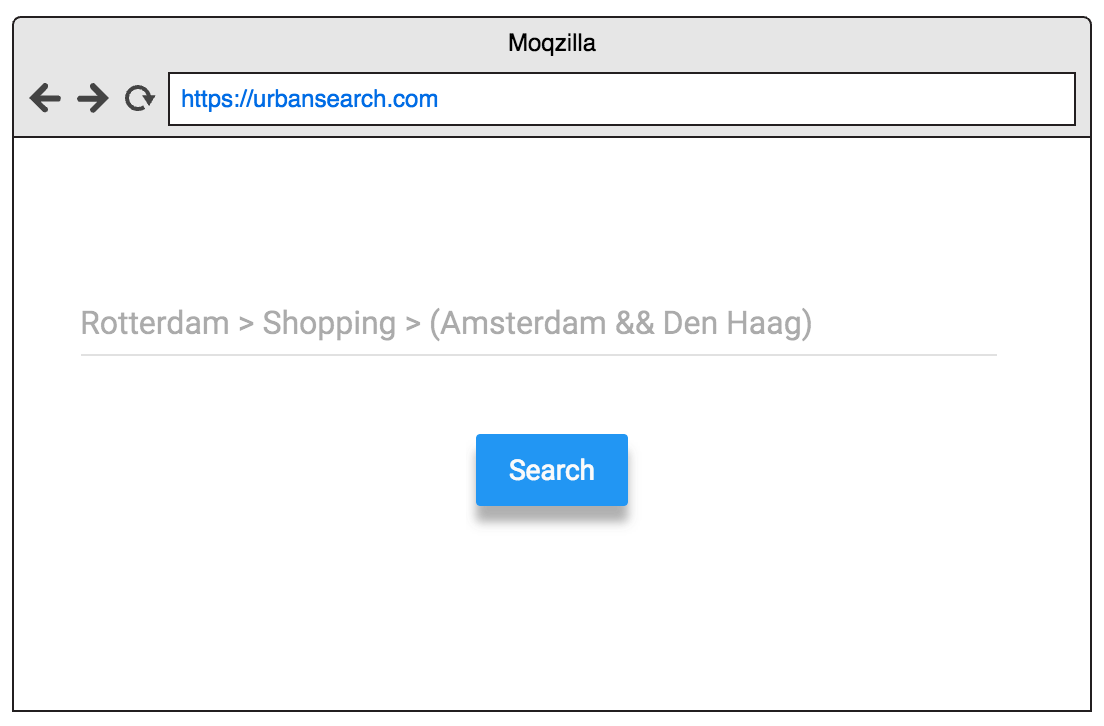
\includegraphics[width=0.75\textwidth]{ql-example}
\caption{Example interface for the query language}
\label{fig:ql-example}
\end{figure}

\subsubsection{Query composer interface}

Another option was to offer the end user a "query composition interface". This interface would have the same possibilities as the former mentioned query language, but should be more intuitive to use for new users. An example of the interface is given in figure \ref{fig:qi-example}.

\begin{figure}[h]
\centering
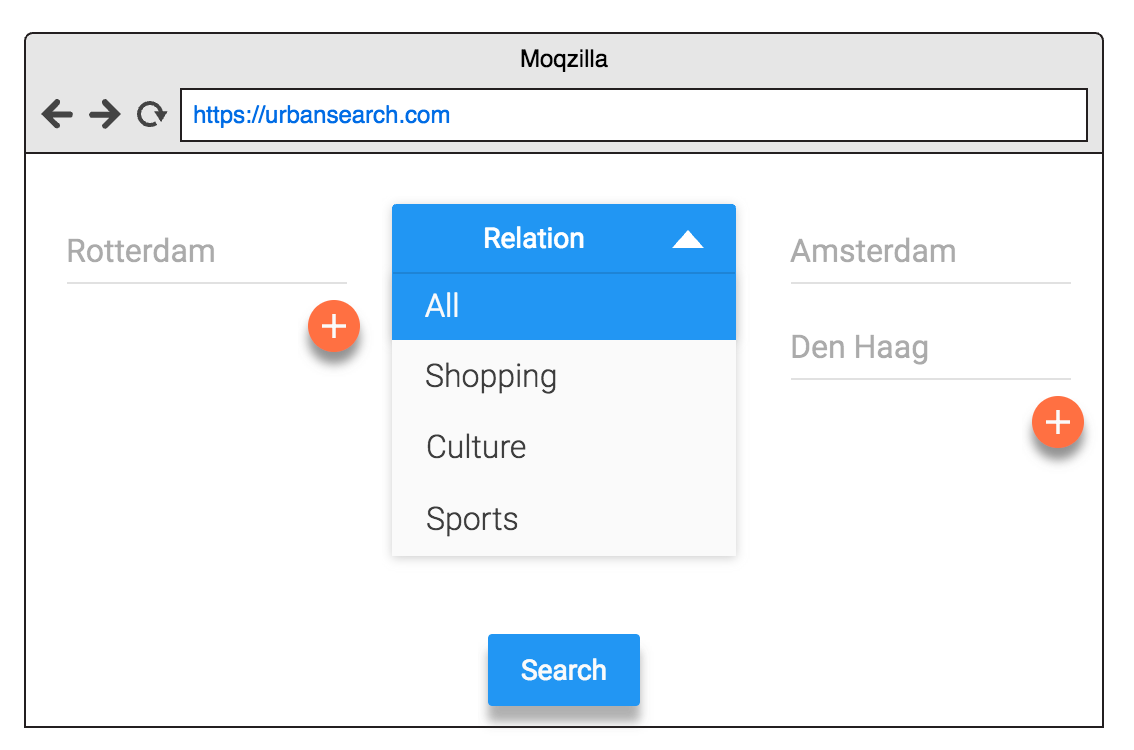
\includegraphics[width=0.75\textwidth]{qi-example}
\caption{Example of a query composer interface}
\label{fig:qi-example}
\end{figure}

\subsubsection{Interactive search}

The last option we investigated was an interactive approach to querying data. This means that the user interacts with a map containing relations and cities. A very simple example is given in figure \ref{fig:ii-example}.


\begin{figure}[h]
\centering
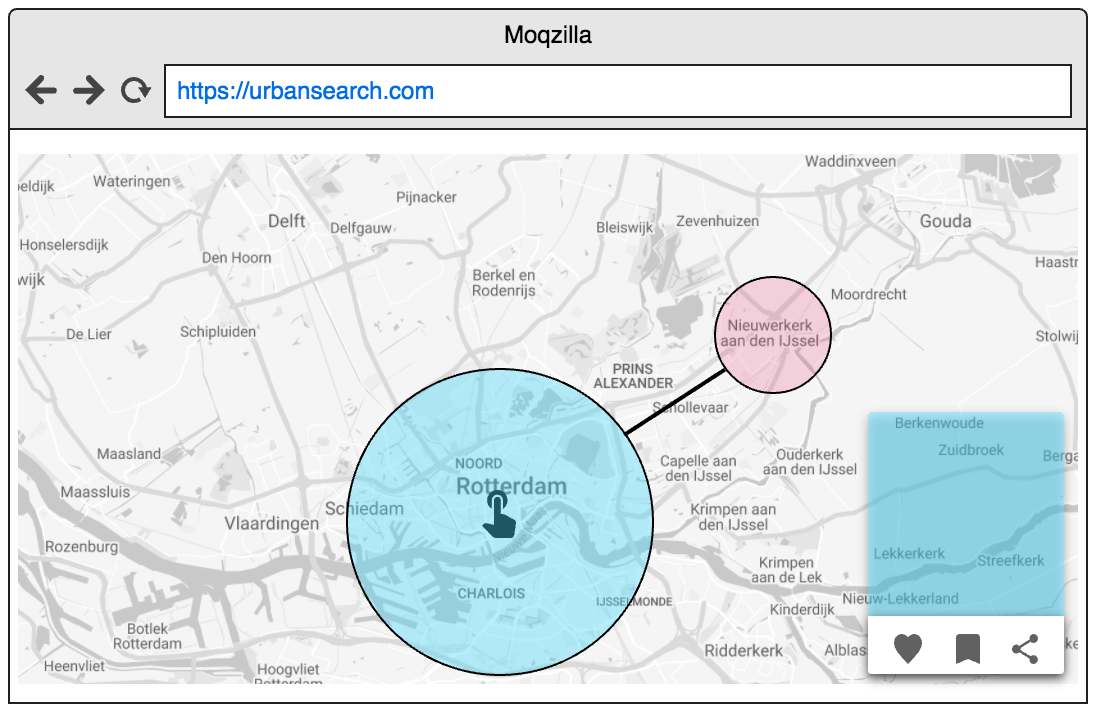
\includegraphics[width=0.75\textwidth]{ii-example}
\caption{Example of an interactive map}
\label{fig:ii-example}
\end{figure}

In this setup the user can click on cities and relations on the map which then triggers a query on the Neo4j back-end. The results can be visualised on the map (eg. showing information about the selected city).

\subsubsection{Conclusion}

Together with the client we decided that the best option was to go with the interactive map. This would lead to easy access to the data by the client and would fit better with the flow of use the client envisioned prior to the project. 
Also from the point of view of the researcher using the application, it fits a lot better in his/her work flow. The application is used to analyse and visualise relations between cities, if this can be done directly on the map it speeds up the users use of the system, since it is faster to select cities and relations on the fly. This helps make the application more intuitive since the user is probably more familiar with a map than with a new query language.
The creation of complex queries is also made a lot easier. The user doesn't have to write or compose a complex query in advance but can do it directly on the map. So getting a visual representation of several cities, interconnected with multiple relations, doesn't mean writing or composing a very long query but clicking/selecting cities and relations on the map.
Interaction directly with the map also reduces the need to go to a separate page to enter/compose a query. This speeds up the use of the system by reducing page loads and it interrupts the work flow of the user less.
A final advantage of using an interactive map over raw queries/query composition is that we don't have users entering invalid queries, this leads to less frustration using the system.